\section{Introduction}

%Wind Firm Energy Certificate (FEC) \cite{porrua2010wind} estimation imposes several challenges. First, it is a quantile function of an aleatory quantity, named here on wind capacity factor (WP). Due to its non-dispachable profile, accurate scenario generation models could reproduce a fairly dependence structure in order to the estimation of FEC. Second, as it is a quantile functions, the more close to the extremes of the interval, the more sensitive to sampling error.



Quantile Regression is a powerful tool for measuring quantiles others than the median or predicting the mean. A quantile of a random variable is important in risk measuring, as we can measure the probability of occurrence of extreme events, and in many other fields. While working with energy forecasts, quantile regression can produce interesting results when working with both short term (hourly) or long term (monthly) data. As an example, we present a solar time series for the short term and a wind time series for long term. The first set of data is measured at the location of Tubarao (Brazil) on the year of 2014, while the latter is a dataset of mean power  monthly observations from Icaraizinho (Brazil) between 1981 to 2011 of measured in Megawatts. Figure \ref{fig:boxplots} illustrate the seasonality present in these datasets.

%\begin{figure}[h]
%	\centering
%	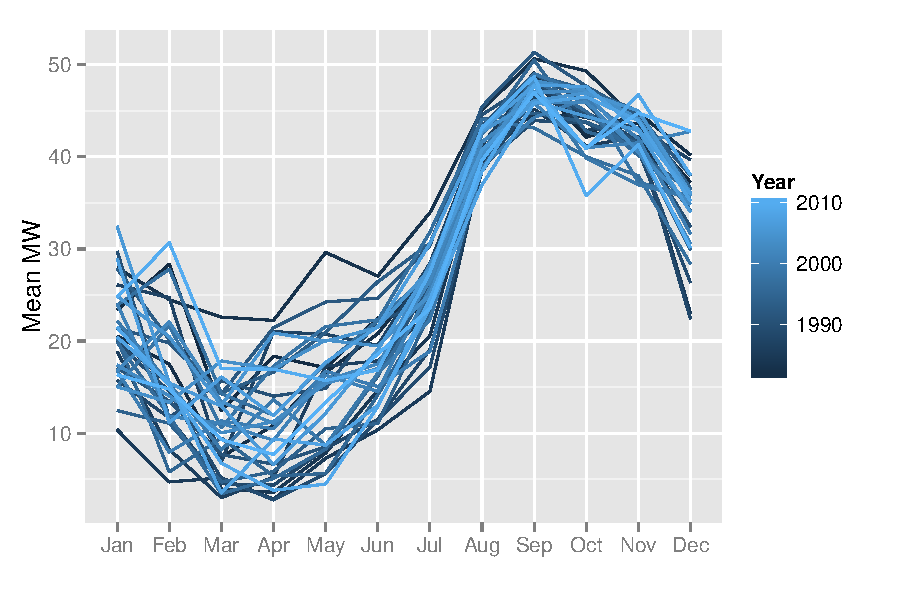
\includegraphics[width=0.8\linewidth]{./Figuras/Icaraizinho/icaraizinho-mensal}
%	\caption{Icaraizinho yearly data. Each serie consists of monthly observations for each year.}
%	\label{fig:icaraizinho-mensal}
%\end{figure}

%
%\begin{figure}
%  \centering
%  \begin{minipage}[t]{1.2\linewidth}
%    \begin{minipage}[t]{0.45\linewidth}
%       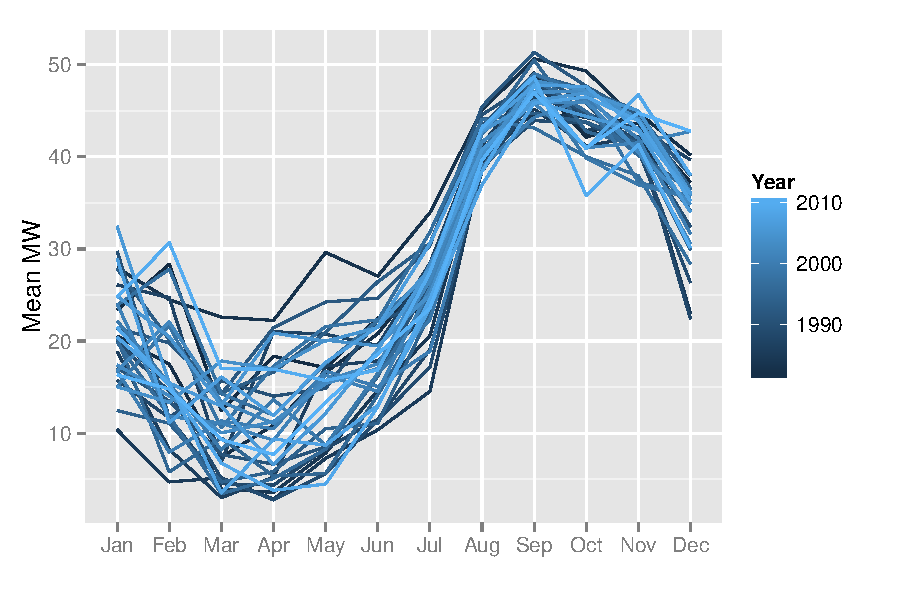
\includegraphics[width=\textwidth]{./Figuras/Icaraizinho/icaraizinho-mensal}
%      	%\caption{Boxplot for each month for the Icaraizinho dataset}
%      	\label{fig:icaraizinho-boxplot}
%    \end{minipage}
%    \begin{minipage}[t]{0.45\linewidth}
%       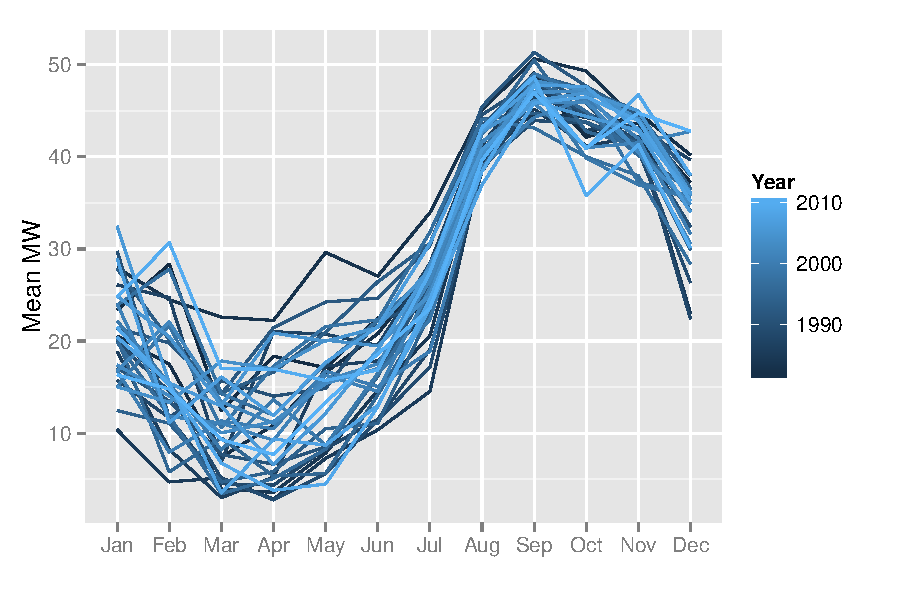
\includegraphics[width=\textwidth]{./Figuras/Icaraizinho/icaraizinho-mensal}
%      	%\caption{Boxplot for each month for the Icaraizinho dataset}
%      	\label{fig:tubarao-boxplot}
%    \end{minipage}
%  \end{minipage}
%  \caption{Relationship between $y_t$ and some chosen lags.}
%  \label{fig:boxplots}
%\end{figure}


In this work, we apply a few different techniques to forecast the quantile function a few steps ahead. The main frameworks we investigate are parametric linear models and a non-parametric regression. We also investigate how to apply quantile estimations to produce an empirical distribution for the $k$-step ahead forecasting by using a nonparametric approach.
%To study our methods performance, we use the mean power monthly data of Icaraizinho, a wind farm located in the Brazilian northeast, and solar.

%The Icaraizinho dataset consists of monthly observations from 1981 to 2011 of mean power measured in Megawatts. The full Icaraizinho serie can be found on the appendices from this article.  As is common in renewable energy generation, there is a strong seasonality component. Figures \ref{fig:icaraizinho-mensal} and \ref{fig:icaraizinho-boxplot} illustrate this seasonality, where we can observe low amounts of power generation for the time span between February and May, and a yearly peek between August and November.

To make good predictions of random variables, one must find good explanatory variables: it can be either autoregressive, exogenous terms or even a deterministic function that repeats itself.
Figure \ref{fig:scatterplot-1lag} shows scatter plots relating $y_t$ with its first lag for both short and long term. We can see that in both of them past values are good explanatory variables to use for forecasting.

\begin{figure}
  \centering
  \begin{minipage}[t]{\linewidth}

    \begin{minipage}[t]{0.45\linewidth}
      %\centering
       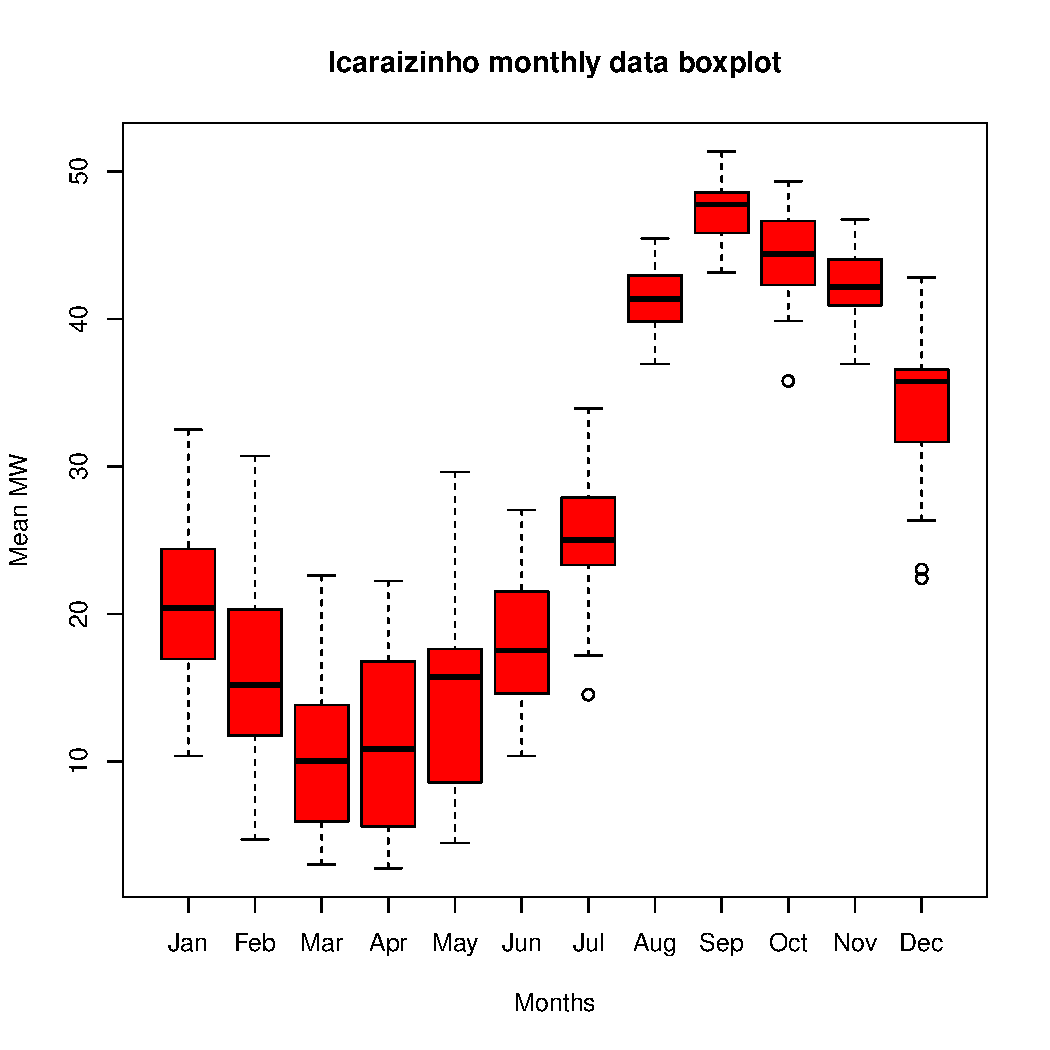
\includegraphics[width=\textwidth]{./Figuras/Icaraizinho/icaraizinho-boxplot}
      	%\caption{Boxplot for each month for the Icaraizinho dataset}
      	\label{fig:icaraizinho-boxplot}
    \end{minipage}
    \begin{minipage}[t]{0.45\linewidth}
      %\centering
       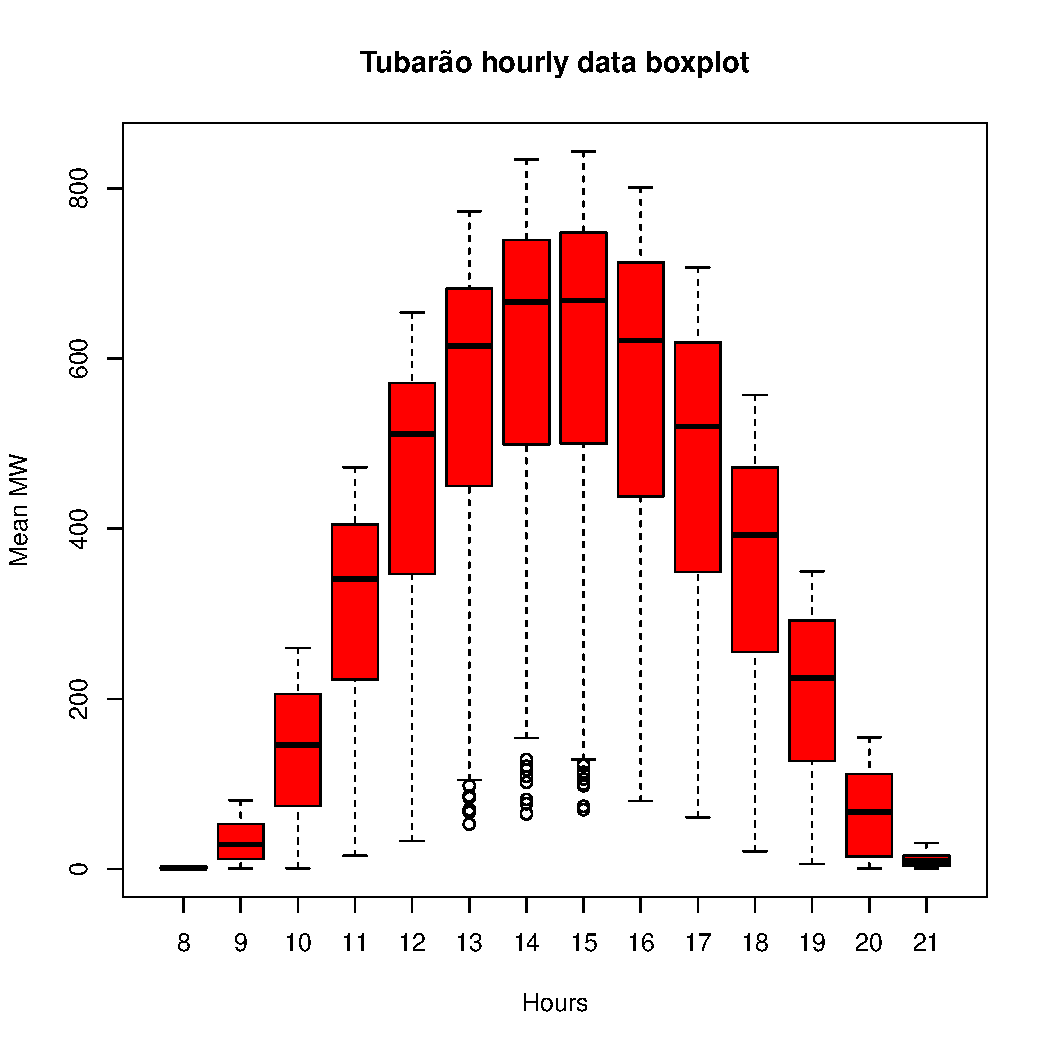
\includegraphics[width=\textwidth]{./Figuras/Solar-exemplos/tubarao-boxplot}
      	%\caption{Boxplot for each month for the Icaraizinho dataset}
      	\label{fig:tubarao-boxplot}
    \end{minipage}
  \end{minipage}
  \caption{Boxplots showing seasonality for monthly and hourly data.}
  \label{fig:boxplots}
\end{figure}



\begin{figure}
  \centering
  \begin{minipage}[t]{\linewidth}
    \centering
    \begin{minipage}[t]{0.45\linewidth}
      \centering     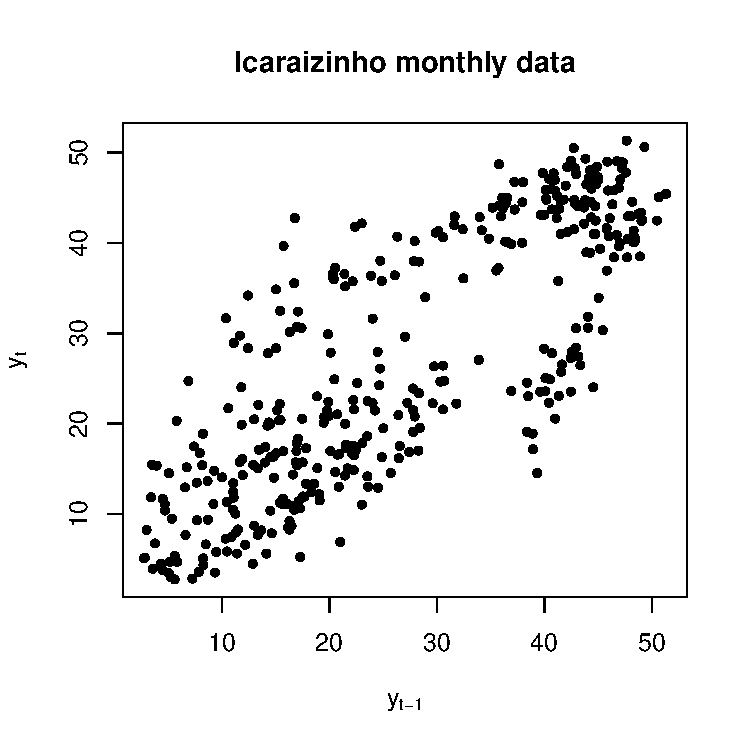
\includegraphics[width=\textwidth]{Figuras/Icaraizinho/scatterplot.pdf}
    \end{minipage}
    \begin{minipage}[t]{0.45\linewidth}
      \centering     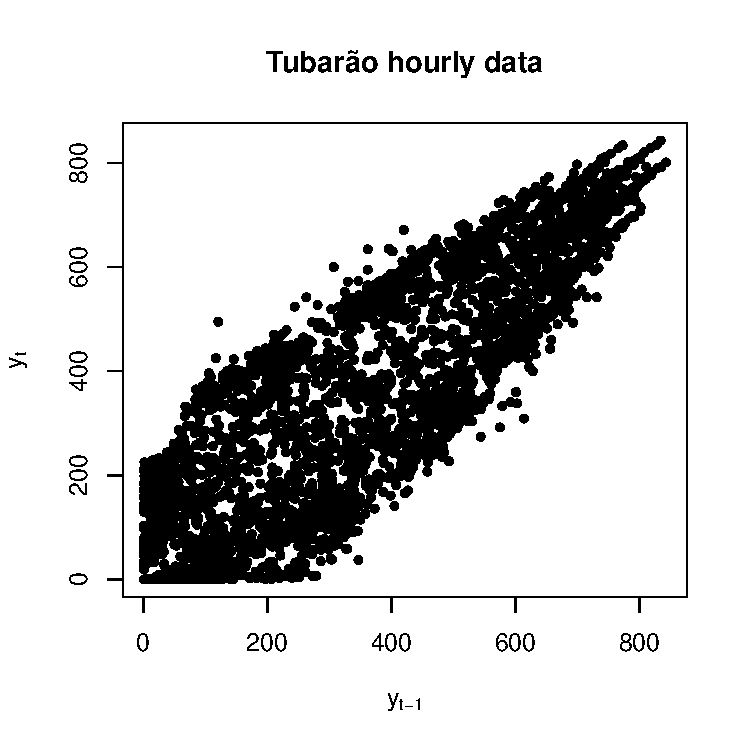
\includegraphics[width=\textwidth]{Figuras/Solar-exemplos/scatterplot}
    \end{minipage}
  \end{minipage}
  \caption{Relationship between $y_t$ and its first lags for two selected series.}
  \label{fig:scatterplot-1lag}
\end{figure}

In contrast to the linear regression model through ordinary least squares (OLS), which provides only an estimation of the dependent variable conditional mean, quantile regression model yields a much more detailed information concerning the complex relationship about the dependent variable and its covariates. Here we denote as parametric linear model the well-known quantile regression model \cite{koenker2005quantile}.

Let $Y$ be a real valued random variable. The quantile function $Q_Y:[0,1] \rightarrow \mathbb{R}$ is defined pointwise by its $\alpha$-quantile, which is given by
\begin{equation}
Q_Y(\alpha) = F_Y^{-1}(\alpha) = \inf\{y: F_Y(y) \geq \alpha\},
\label{eq:quantile-function}
\end{equation}
where $F_Y$ is the distribution function of random variable $Y$ and $\alpha \in [0,1]$. Equation \ref{eq:quantile-function} defines what we call from now on as the quantile function $Q_Y(\cdot)$, in relation to random variable $Y$. In this article, we are interested in a conditional quantile function $Q_{Y|X=x}(\alpha, x)$ (in short, from now on, $Q_{Y|X}(\alpha, x)$), where $X$ can be a vector.

Let $(\Omega, \mathcal{F}, P)$ be a probability space. The conditional quantile function can be found as the result of the following optimization problem:
\begin{eqnarray}
Q_{Y|X}(\alpha,x)\quad & \in\quad\underset{q_\alpha(\cdot)}{\text{arg min}}\, &
(1-\alpha)\int_{\omega \in \Omega}|Y(w)-q_\alpha(X(w))|^{-}P(dw) \label{eq:optim-continuous}
 \\ & & + (\alpha)\int_{\omega \in \Omega}|Y(w)-q_\alpha(X(w))|^{+}P(dw) \nonumber
\end{eqnarray}

\begin{equation}
  q_\alpha  \in \mathcal{Q},
\end{equation}
where $A$ is a set containing a sequence of probabilities  $\alpha_i$ such that $0 < \alpha_1 < \alpha_2 < \dots < \alpha_Q < 1$. This set represents a finite discretization of the interval $[0,1]$. These values must be close enough so that $Q_{Y|X}(\alpha)$ has a precise representation. The argument of optimization problem described on equation \ref{eq:optim-continuous} is the function $q_\alpha$, which belongs to a function space $\mathcal{Q}$. We might have different assumptions for the space $\mathcal{Q}$, depending on the type of function we want to find for $q_\alpha$. A few properties, however, must be achieved by our choice. The conditional quantile function $Q_{Y|X}(\alpha)$ must be monotone on $\alpha$, and its first derivative must be limited.

In this work, we use the sample quantile,  where we calculate the optimization based on a finite number of observations, instead of integrating over all domain of random variable $Y$. For the specific case where the random variable is a time series $y_t$, quantiles are estimated from a $n$ size sample of observations of $y_t$ and a explanatory variable $x_t$ for each $t$, such that our random sample is formed by the sequence $\{y_t,x_t \}_{t=1}^n$. To estimate the $\alpha$-quantile from a sample, we change \ref{eq:optim-continuous} for the following optimization problem:
\begin{equation}
\hat{Q}_{Y|X}(\alpha,x)\quad \in\quad\underset{q_\alpha(\cdot)}{\text{arg min}}\,\sum_{t=1}^{n}\alpha|y_{t}-q_\alpha(x_t)|^{+}+\sum_{t=1}^{n}(1-\alpha)|y_{t}-q_\alpha(x_t)|^{-},
\label{eq:linear-model}
\end{equation}
\begin{equation}
  q_\alpha  \in \mathcal{Q},
\end{equation}
where $q_\alpha(x_t)$ is the estimated quantile value at a given time $t$ and $|x|^+=\max\{0,x\}$ and $|x|^-=-\min\{0,x\}$. The solution from the above problem is an estimator $\hat{Q}_{Y|X}$ for the quantile function $Q_{Y|X}$.

To model this problem as a Linear Programming problem, thus being able to use a modern solver to fit our model,  we create variables $\varepsilon^+_t$ e $\varepsilon^-_t$ to represent $|y-q(x_t)|^+$ and $|y-q(x_t)|^-$, respectively. The optimal argument $q_\alpha^*(\cdot)$ on the Linear Programming problem \ref{eq:qar-general} is the estimated $\alpha$-quantile for the given random sample.
\begin{equation}
\begin{aligned}\min_{q_\alpha (\cdot),\varepsilon_{t}^{+}, \varepsilon_{t}^{-}} & \sum_{t=1}^{n}\left(\alpha \varepsilon_{t}^{+}+(1-\alpha)\varepsilon_{t}^{-}\right) & \\
\mbox{s.t. } & \varepsilon_{t}^{+}-\varepsilon_{t}^{-}=y_{t}-q_\alpha(x_{t}), & \qquad\forall t \in \{1,\dots,n\},\\
& \varepsilon_t^+,\varepsilon_t^- \geq 0, & \qquad \forall t \in \{1,\dots,n\}.
\end{aligned}
\label{eq:qar-general}
\end{equation}

One of our goals with quantile regression is to estimate a quantile function $\hat{Q}_{Y|X}$ of a given real valued random variable $X$ from a sequence of quantiles $q_{\alpha_1}(x_t) \leq q_{\alpha_2}(x_t) \leq \dots \leq q_{\alpha_{|A|}}(x_t)$, with $0 < \alpha_1 < \alpha_2 < \dots < \alpha_{|A|} < 1$, for any given $t$.
The process of fitting $\hat{Q}_Y$ is by mapping every $\alpha_i$ with its estimated quantile $\hat{q}_{\alpha_i}(x_t)$.
When this sequence of chosen $\alpha_i$ is thin enough, we have a good approximation of $Q_{Y|X}$.
Thus, the distribution found for $Y$ is nonparametric, as no previous assumptions are made about its shape, and its form is fully recovered by the data we have.

A typical problem, however, arises when working with quantile regression. When quantiles are estimated independently, it is possible to find $q_{\alpha}(x_t) > q_{\alpha'}(x_t)$, for a given $t$, when $\alpha_1 < \alpha_2$. An example can be seen on Figure \ref{fig:crossing-quantiles}, where quantiles $\alpha = 0.95$ and $\alpha = 0.9$ cross. This problem, called \textit{crossing quantiles}, can be prevented by estimating all quantiles with a single minimization problem.
\begin{figure}
	\centering
	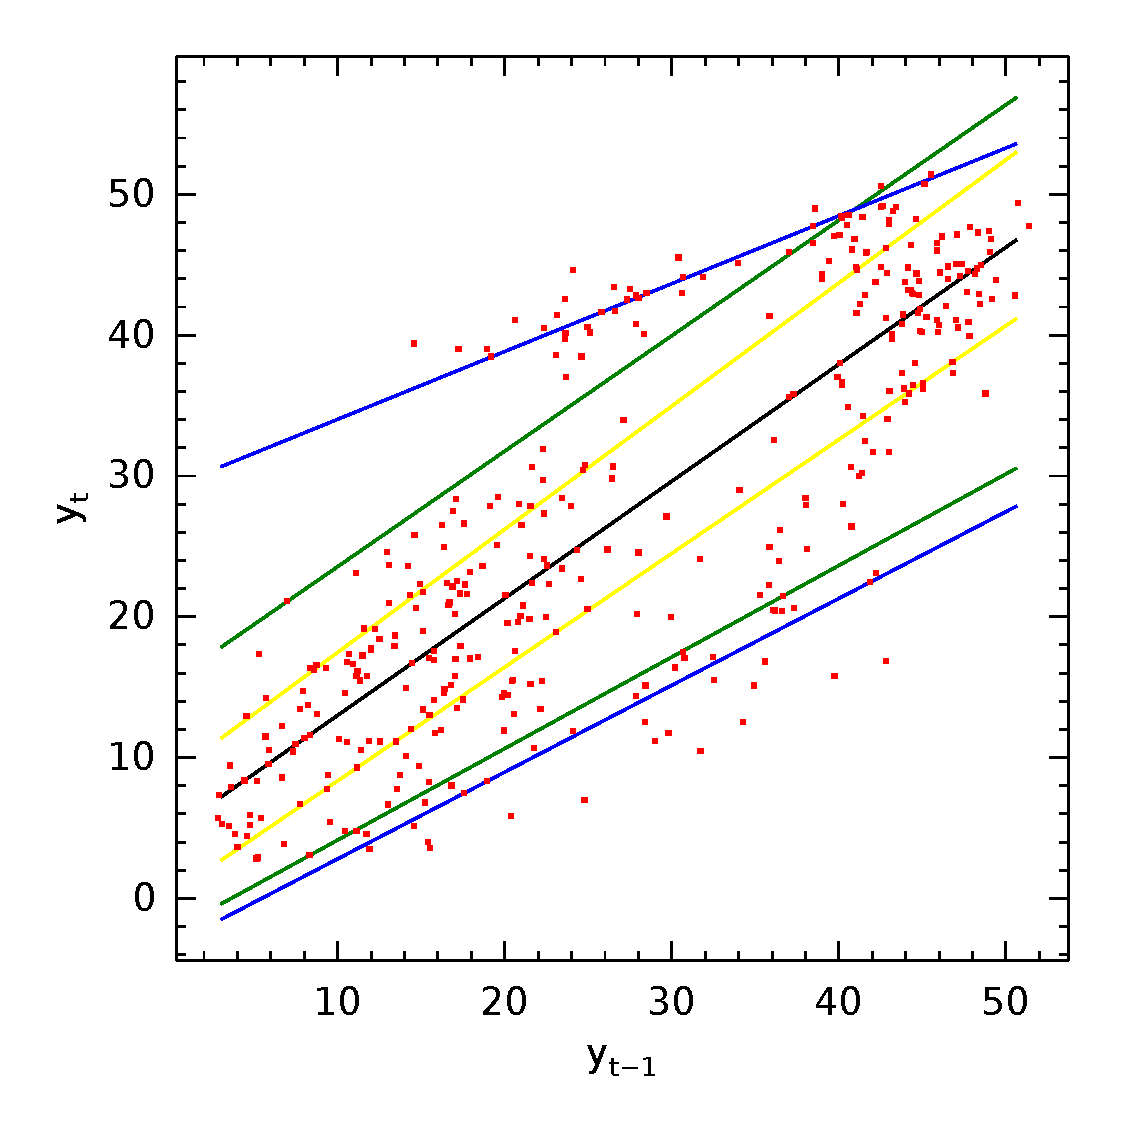
\includegraphics[width=0.6\linewidth]{./Figuras/npqar/icaraizinho-crossing-200}
	\caption{Linear quantile estimator with crossing quantiles for $\alpha = 0.95$ and $\alpha = 0.9$}
	\label{fig:crossing-quantiles}
\end{figure}

 Let $T_n = \{1, 2, \dots, n\}$. In order to estimate all quantiles simultaneously, the new objective function will be the sum of all individual objective functions, as well as include all constraints from all individual problems. The only difference is the inclusion of an equation to guarantee that quantiles won't cross. When modifying problem \ref{eq:qar-general} to account for all quantiles, we have the following new problem:
\begin{eqnarray}
\label{eq:non-crossing-quantiles1}
\min_{q_\alpha(\cdot),\varepsilon_{t,\alpha}^{+}, \varepsilon_{t,\alpha}^{-}} &  \sum_{\alpha \in A} \sum_{t \in T_n}\left(\alpha \varepsilon_{t,\alpha}^{+}+(1-\alpha)\varepsilon_{t,\alpha}^{-}\right) &  \\
\mbox{s.t. } & \varepsilon_{t,\alpha}^{+}-\varepsilon_{t,\alpha}^{-}=y_{t}-q_\alpha(x_{t}), & \qquad\forall t \in T_\tau,\forall \alpha \in A,\\
& \varepsilon_{t,\alpha}^+,\varepsilon_{t,\alpha}^- \geq 0, & \qquad\forall t \in T_\tau,\forall \alpha \in A,\\\label{eq:non-crossing-constraint}
& q_{\alpha}(x_t) \leq q_{\alpha'}(x_t), & \qquad \forall t \in T_\tau, \forall (\alpha, \alpha') \in AxA,  \alpha' \geq \alpha,
\end{eqnarray}
where constraint \ref{eq:non-crossing-constraint} assures that no lower quantile will have a bigger value than a higher quantile.




The next section discusses with bigger details how to fit a distribution function $Q_{Y|X}(\alpha,x)$ from a sequence of estimated quantiles, as well as showing two different strategies to estimate them: linear models and nonparametric models. In the former, $q_\alpha$ is a linear function of an explanatory variable $x_t$.
In the latter, we let $q_\alpha(x_t)$ assume any functional form. To prevent overfitting, however, we penalize the function's roughness by incorporating a penalty on the second derivative.

In section \ref{sec:simulation} we investigate how to simulate $S$ scenarios of $y_t$, considering a linear model and errors $\varepsilon_t$ for which the distribution is unknown. To address this issue, we use quantile linear regression to calculate a thin grid of quantiles and fit a distribution function $\hat{F}_{y_t}$. This function will be used to simulate the innovations on the model.
